% !TEX root = index.tex

%basic AMS packages
\documentclass[reqno,letter, 11pt,twoside]{article}
\usepackage{amsmath}
\usepackage{amsthm}
\usepackage{amssymb}
\usepackage{hyperref}
\hypersetup{
	colorlinks = true,
	linkcolor = blue,
	anchorcolor = blue,
	citecolor = blue,
	filecolor = blue,
	urlcolor = blue
}
\usepackage{epigraph}
\usepackage{mathpazo}
\usepackage{tcolorbox}
\usepackage[margin=1in,includehead,includefoot]{geometry}
\usepackage{fancyhdr}
  \pagestyle{fancy}
  \fancyhf{}
  \fancyhead[LO]{The Quantum Spring}
  \fancyhead[RE]{Apurva}
  \fancyhead[LE]{Mathcamp}
  \cfoot{\thepage}

\usepackage{graphicx}
  \graphicspath{ {images/} }
\usepackage{float}
\usepackage{subcaption}
\usepackage{color}
\usepackage{mdframed}
\usepackage{enumitem}
  \setlist[enumerate]{label=\emph{\alph*})}% global settings, for all lists
\usepackage{tikz}
\usepackage[all,cmtip]{xy}
\usepackage{multicol}
% \renewcommand{\thefootnote}{\fnsymbol{footnote}}

% \makeatletter
% \@addtoreset{footnote}{section}
% \makeatother

%for setting the equation number to sync with the theorem numbers
\numberwithin{equation}{section}
\newcommand{\hint}[1]{\footnote{\raggedleft\rotatebox{180}{Hint: #1\hfill}}}

%How does latex not have these?
\DeclareMathOperator{\Ad}{Ad}
\DeclareMathOperator{\ad}{ad}
\DeclareMathOperator{\tr}{tr}
\DeclareMathOperator{\Tr}{Tr}
\DeclareMathOperator{\Hom}{Hom}
\DeclareMathOperator{\maps}{Maps}
\DeclareMathOperator{\im}{im}
\DeclareMathOperator{\rank}{rank}
\DeclareMathOperator{\coker}{coker}
\DeclareMathOperator{\Exists}{\exists}
\DeclareMathOperator{\Forall}{\forall}
\DeclareMathOperator{\res}{Res}
\DeclareMathOperator{\mor}{Res}

%simple operators which can be pretty useful
\newcommand{\pr}[2][\:]{\frac{\partial #1}{\partial #2}}
\newcommand{\innerp}[2]{\langle #1, #2 \rangle}
\newcommand*\conj[1]{\overline{#1}}
\newcommand*\norm[1]{\lVert #1 \rVert}

\theoremstyle{plain}
\newtheorem{thm}{Theorem}[section]
\newtheorem{prop}[thm]{Proposition}
\newtheorem{lem}[thm]{Lemma}
\newtheorem{cor}[thm]{Corollary}


\theoremstyle{definition}
\newtheorem{definition}[thm]{Definition}
\newtheorem{example}[thm]{Example}
\newtheorem{remark}[thm]{Remark}
\newtheorem{ans}[thm]{Ans.}

\newcounter{q}
\newtheorem{question}[q]{Question.}
\definecolor{light-gray}{gray}{0.95}
\newenvironment{ques}
{
	\begin{tcolorbox}[colback=light-gray,arc=0pt,outer arc=0pt,boxrule=0.5pt]
	 \begin{question}
			}
			{
		\end{question}
	\end{tcolorbox}
}

%Real numbers, complex numbers, etc.
\newcommand{\R}{\mathbb{R}}
\newcommand{\C}{\mathbb{C}}
\newcommand{\Z}{\mathbb{Z}}
\newcommand{\Q}{\mathbb{Q}}
\newcommand{\F}{\mathbb{F}_2}
\newcommand{\U}{\mathcal{U}}
\newcommand{\V}{\mathcal{V}}
\renewcommand{\L}{\mathcal{L}}
\renewcommand{\P}{\mathcal{P}}
\newcommand{\B}{\mathcal{B}}

\usepackage{wrapfig}
\usepackage[makeroom]{cancel}

\title{The Quantum Spring}
\author{\small{Apurva Nakade}}
\date{}
\begin{document}
\maketitle
\vspace{-2em}
\epigraph{Not only is the universe stranger than we imagine, it is stranger than we can imagine.}{J.B.S. Haldane}
\vspace{-2em}
\tableofcontents

\section{The Mass-Spring System}
\subsection{The Classical Spring}
A mass-spring system (also called a harmonic oscillator) consists of a point mass $m$ attached to a spring with spring constant $k$. We'll assume that there is no external force or friction. In Newtonian mechanics the laws of motion are given by the equations,
\begin{align*}
	F &= m \dfrac{d^2 x }{dt^2}\\
	F &= -kx
\end{align*}
\begin{wrapfigure}{r}{0.5\textwidth}
		\centering
		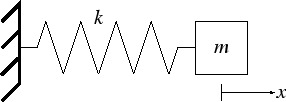
\includegraphics[height=1.5cm]{mass-spring}
	\end{wrapfigure}
Combining these we get $\frac {d^2 x }{dt^2} = -\frac{k}{m}x$ which has the solutions
\begin{align}
	\label{eq:classical_solutions}
	x = A \sin (\omega t) + B \cos(\omega t)
\end{align}
where $\omega^2=k/m$ and $A, B$ are constants which depend on the initial conditions. The constant $\omega$ is the frequency of oscillation. We can rewrite this as a conservation of energy equation
\begin{align}
	\label{eq:energy_mass_spring}
	\dfrac{1}{2} \left(\dfrac{p^2}{m} + k x^2\right) = E
\end{align}
where $p = m \frac{dx}{dt}$ is the momentum and $E$ is total energy of the system which is constant.

\begin{ques}
	Show that the solutions \eqref{eq:classical_solutions} satisfy the energy conservation equation \eqref{eq:energy_mass_spring}.
\end{ques}

\subsection{Quantizing a Classical System}
On the microscopic level, this system is seen in a diatomic molecule like $H_2$. If we look at the system from the frame of reference of the center of mass then up to a first approximation the atom behaves like a mass-spring system (plus some rotational motion). One can measure the energy of this mass-spring system and it turns out that the energy is quantized, more specifically the energy of this mass-spring system only takes values of the form
\begin{align*}
	c(n + 1/2)
\end{align*}
where $c$ is a positive real constant that depends on the molecule and $n$ is a non-negative integer!

The Newtonian model on the other hand predicts that we should see a continuous spectrum of possible energy values. As the model does not agree with experiments we need to discard this model and come up with a new model i.e. quantum mechanics. The current model for a quantum mechanical analogue of a classical mechanical system is the following:\\

The entire information about the state of a system is contained in a \textbf{wavefunction} which is simply a time-dependent complex valued function
\begin{align*}
	\psi (x, t)
\end{align*}
Further, we think of these wavefunctions as living in the $\C$-vector space of all complex valued functions.\footnote{As it is stated this is false. We need to impose several analytic conditions on the space of functions for this to make sense. The usual candidate is the $L^2$-space of functions.}\\

In this model, the \emph{observable} quantities like position, momentum, angular momentum, energy etc. are \textbf{linear operators} on this vector space. We'll the denote linear operators as $\hat{-}$;
\begin{align*}
	 \hat{x} &= \mbox{position operator}\\
 \hat{p} &= \mbox{momentum operator}  \\
\hat{E} &= \mbox{energy operator}
\end{align*}

To find equations of motion we replace the observable quantities with the corresponding operators in the energy conservation equation. For the mass-spring system this is Equation \ref{eq:energy_mass_spring} which gives us the \textbf{Schrodinger Equation}

	\begin{align}
		\label{eq:Schrodinger}
		\dfrac{1}{2} \left(\dfrac{\hat{p} \circ \hat{p}}{m} + k \hat{x} \circ \hat{x}\right)\psi = \hat{E} \psi
	\end{align}
where we're solving for $\psi$ (which is a function of $x, t$).

Finally, we need to find the \emph{right} linear operators, this is again a choice we have to make in our model. For the time independent or steady state\footnote{This is saying that no external force is being applied to the system and the system has stabilized into an equilibrium state. For example, standing waves are examples of steady states of the classical waves-on-a-string system.} mass-spring system these are
\begin{align*}
	\hat{x} &= x \cdot (-) \quad(\mbox{ multiplication by } x) \\
	\hat{p} &= -i \hbar \dfrac{d}{d x} \\
		\hat{E} &= \lambda \cdot (-) \quad(\mbox{ multiplication by a fixed positive real number})
\end{align*}
where $i = \sqrt{-1}$ and $\hbar$ is a physical constant called the \textbf{Planck's constant}.\\

\noindent \textbf{Aside: } This is only half the story. Here we're only talking about finding a mathematical model, in particular, a differential equation, for describing the quantum world. There still needs to be an interpretation of this model in terms of physically observable quantities to connect the model to experiments. This in itself is a long and beautiful story which you should explore by yourself.\\

Being mathematicians we'll assume that $m = k = \hbar = 1$ so that the time-independent Schrodinger equation \eqref{eq:Schrodinger} for a mass-spring system becomes
\begin{align*}
	\dfrac{1}{2} \left({\left(-i \dfrac{d}{d x}\right) \circ \left(-i \dfrac{d}{d x}\right)} + k x^2\right)\psi = \lambda \psi \\
	 \dfrac{1}{2} \left(-\dfrac{d^2 \psi}{d x^2} + {x}^2 \psi \right) = \lambda \psi
\end{align*}
Define the \textbf{Schrodinger operator} to be
\begin{align*}
		\hat{H} := \dfrac{1}{2}	\left(- \dfrac{d^2}{d x^2} + {\hat{x}}^2 \right)
\end{align*}
so that we can rewrite the Schrodinger equation simply as
\begin{align*}
	\hat{H} \psi = \lambda \psi
\end{align*}
But notice that the solutions to this are simply the eigenvectors of $\hat{H}$!!!
\begin{prop}
		The solutions to the time-independent Schrodinger equation are precisely the eigenvalues and eigenvectors of the Schrodinger operator.
\end{prop}







\section{Linear Algebra}

\subsection{The Schrodinger Operator}
Thus we've reduced a physics problem to a linear algebra one (yay!). We'll now focus entirely on the Schrodinger operator. The operator $2\hat{H}$  should not be very far from the operator $(-d/dx + x)(d/dx + x)$, more precisely
\begin{align*}
	&\left(-\dfrac{d}{dx} + \hat{x}\right) \circ \left(\dfrac{d}{dx} + \hat{x} \right)\psi \\
	&=\left(-\dfrac{d}{dx} + \hat{x}\right) \circ \left(\dfrac{d \psi}{dx} + x \psi \right) \\
	&= -\dfrac{d}{dx}\left( \dfrac{d \psi}{dx} + x \psi \right) + \hat{x} \left( \dfrac{d \psi}{dx} + x \psi \right) \\
	&= -\dfrac{d^2 \psi}{dx^2} -\dfrac{d}{dx} \left(x \psi \right) + x\dfrac{d \psi}{dx} + x^2 \psi \\
	&= -\dfrac{d^2 \psi}{dx^2} -\psi - \cancel{x\dfrac{d\psi}{dx}} + \cancel{x\dfrac{d \psi}{dx}} + x^2 \psi \\
	&= 2\hat{H} \psi - \psi
\end{align*}

\begin{definition}
	Define the \textbf{creation} operator $\hat{C}$ and \textbf{annihilation} operator $\hat{A}$ as
	\begin{align*}
		\hat C &:= \dfrac{1}{\sqrt{2}}\left(-\dfrac{d}{dx} + \hat{x}\right)
		=\dfrac{1}{\sqrt{2}}\left(-i \hat{p} + \hat{x}\right) \\
			\hat A &:= \dfrac{1}{\sqrt{2}}\left(\dfrac{d}{dx} + \hat{x}\right)
		=\dfrac{1}{\sqrt{2}}\left(i \hat{p} + \hat{x}\right)
	\end{align*}
\end{definition}
\noindent By the above derivation we have
\begin{align*}
	\hat{H} &= \hat{C} \hat{A} + \frac{1}{2}
\end{align*}
The operators $\hat{H}, \hat{C}, \hat{A}$ are the generating elements of an algebra called the \textbf{Weyl algebra} which we'll now analyze.











\subsection{Lie Brackets}
If two operators $\hat{M}$ and $\hat{N}$ commute and if $\psi$ is an eigenvector of $\hat{M}$ with eigenvalue $\lambda$ then
\begin{align*}
	\hat{M} \hat{N} \psi
	&= \hat{N} \hat{M} \psi \\
	&= \lambda \hat{N} \psi
\end{align*}
\begin{prop}
	If $\hat{M}$ and $\hat{N}$ commute and $\psi$ is an eigenvector of $M$ then so is $\hat{N} \psi$ with the same eigenvalue.
\end{prop}

What happens if they don't commute? The notation of Lie (pronounced \emph{lee}) brackets allows us to analyze this systematically.
Lie  brackets measure the failure of commutativity of operators.
\begin{definition}
	For linear operators $\hat{M}, \hat{N}$ on a $\C$-vector space, the \textbf{Lie bracket} is defined as
	\begin{align*}
		[\hat{M}, \hat{N}] := \widehat{M} \circ \widehat{N} - \widehat{N} \circ \widehat{M}
	\end{align*}
\end{definition}

\begin{ques}
	For linear operators $\hat{M}, \hat{N}, \hat{P}$ prove the following identities.
	\begin{enumerate}
		\item $[\hat{M}, \hat{M}] = 0$
		\item $[\hat{M}, \hat{N}] = -[\hat{N}, \hat{M}]$
		\item $[\hat{M}, c \hat{N} + \hat{P}] = c[\hat{M}, \hat{N}] + [\hat{M}, \hat{P}]\quad $ where $c$ is a complex number
		\item $[\hat{M}, [\hat{N}, \hat{P}]] + [\hat{N}, [\hat{P}, \hat{M}]] + [\hat{P}, [\hat{M}, \hat{N}]] = 0$
	\end{enumerate}
	The last identity is called the \textbf{Jacobi identity}.
\end{ques}

Suppose $\psi$ is an eigenvector of a linear operator $\hat{M}$ and let $\hat{N}$ be another linear operator. If we no longer have commutativity then
\begin{align}
	\label{eq:commutator_eigenvalue}
	\begin{split}
		\hat{M} \hat {N} \psi
		&= [\hat{M}, \hat{N}] \psi + \hat{N} \hat{M} \psi \\
		&= [\hat{M}, \hat{N}] \psi + \lambda \hat{N}  \psi
	\end{split}
\end{align}
This is as far as we can get in full generality. We'll now specialize to the operators that are relevant to us. Let us find the Lie brackets.
\begin{align*}
	[\hat{x}, \hat{p}] \psi
	&= \hat{x} \circ \hat{p} (\psi) - \hat{p} \circ \hat{x} (\psi) \\
	&= -i x \dfrac{d \psi}{dx} + i \dfrac{d}{dx}(x \psi) \\
	&= -\cancel{i x \dfrac{d \psi}{dx}} + \cancel{i x\dfrac{d\psi}{dx}} + i \psi \\
	&= i \psi \\
	\Rightarrow [\hat{x}, \hat{p}] = i
\end{align*}
This is the famous non-commutativity relation that leads to the Heisenberg's Uncertainty Principle. For the creation and annihilation operators we get,
\begin{align*}
	[\hat{C}, \hat{A}] \psi
	&= \left[\dfrac{1}{\sqrt{2}}\left(-i \hat{p} + \hat{x}\right), \dfrac{1}{\sqrt{2}}\left(i \hat{p} + \hat{x}\right)\right] \\
	&= \dfrac{1}{2}[-i \hat{p}, \hat{x}] + \dfrac{1}{{2}}[\hat{x},i \hat{p}] \\
	&= \dfrac{1}{{2}}[\hat{x},i \hat{p}] + \dfrac{1}{{2}}[\hat{x},i \hat{p}] \\
	&= i [\hat{x},\hat{p}] \\
	&= -1
\end{align*}

\begin{ques}
	\label{q:commutivity_relations}
	Show that (you'll need to use the Jacobi identity for this problem)
	\begin{align*}
		[\hat{H}, \hat{C}] &= \hat{C} \\
		[\hat{H}, \hat{A}] &= -\hat{A}
\end{align*}
\end{ques}

\noindent If $\psi$ is an eigenvector of $\hat{H}$ with eigenvalue $\lambda$ then using equation \eqref{eq:commutator_eigenvalue} and Question \ref{q:commutivity_relations} we get
\begin{align*}
	\begin{aligned}
		\hat{H} \hat {C} \psi
		&= [\hat{H}, \hat{C}] \psi + \lambda \hat{C}  \psi \\
		&= \hat{C} \psi + \lambda \hat{C}  \psi \\
		&= (\lambda + 1)\hat{C} \psi
	\end{aligned} &&
	 \begin{aligned}
		\hat{H} \hat {A} \psi
		&= [\hat{H}, \hat{A}] \psi + \lambda \hat{A}  \psi \\
		&= -\hat{A} \psi + \lambda \hat{A}  \psi \\
		&= (\lambda - 1)\hat{C} \psi
	\end{aligned}
\end{align*}
Thus we have shown that
\begin{thm}
	\label{thm:shifts}
	If $\psi$ is an eigenvector of $\hat{H}$ with eigenvalue $\lambda$ then so are
	 \footnote{There is a mistake in this theorem. Can you find it?}
	\begin{align*}
		&\hat{C} \psi \mbox{ with eigenvalue } \lambda + 1  \mbox{ and} \\
		&\hat{A} \psi \mbox{ with eigenvalue } \lambda - 1.
	\end{align*}
\end{thm}
This is why the operator $\hat{C}$ and $\hat{A}$ are called creation and annihilation operators, as they create and destroy {energy}. When we're dealing with actual quantum systems, this increase/decrease in energy is realized by an absorption/emission of a mass-less particle like a photon.

\section{Back to Physics}

This is as far as we can get by analyzing just the operators $\hat{H}, \hat{C}, \hat{A}$ abstractly. Going back to physics, we want $\lambda$ to be non-negative as $\lambda$ represents the total energy of the system. But if $\psi$ is an eigenvector with eigenvalue $\lambda$ then so is $\hat{C}^k \psi$ which has eigenvalue $\lambda-k$ and we can make this negative by choosing a large $k$. So if everything we did above is mathematically correct then we're seeing that there are negative energy states for every quantum mass-spring system.

Hmmm.

This is brings us to the mistake in Theorem \ref{thm:shifts}. The vectors $\hat{C} \psi$ and $\hat{A} \psi$ can be eigenvectors only if they are \textbf{non-zero}. Thus we can restate the theorem as
\begin{thm}
	If $\psi$ is an eigenvector of $\hat{H}$ with eigenvalue $\lambda$ then so are
	 \footnote{There is a mistake in this theorem. Can you find it?}
	\begin{align*}
		&\hat{C} \psi \mbox{ with eigenvalue } \lambda + 1  \mbox{ {\bf if $\hat{C} \psi \neq 0$} and} \\
		&\hat{A} \psi \mbox{ with eigenvalue } \lambda - 1 \mbox{ {\bf if $\hat{A} \psi \neq 0$}}.
	\end{align*}
\end{thm}

Thus we cannot use Theorem \ref{thm:shifts} to create eigenvectors with negative eigenvalues if $\hat{A} \psi_0 = 0$. For this eigenvector, the energy equals
\begin{align*}
	\hat{H} \psi_0
	&= (\hat{C} \hat{A} + 1/2) \psi_0 \\
	&= \hat{C} \cancel{\hat{A} \psi_0} + 1/2 \psi_0 \\
	&= \frac{1}{2} \psi_0
\end{align*}
This eigenvector is called the \textbf{ground state}.
Every other eigenvalue is $n + 1/2$ for some positive integer $n$, which corresponds to the eigenvector $\hat{C}^n \psi_0$. This indeed agrees with experiments, and so we can say that this model of quantum mechanics is \emph{not incorrect}.

We can find the ground state explicitly by solving
\begin{align*}
	&\hat{A} \psi = 0 \\
	\Rightarrow\quad &\left( \frac{d}{dx} + x\right) \psi = 0 \\
	\Rightarrow\quad &\frac{d\psi}{dx} + x\psi = 0 \\
	\Rightarrow\quad &\psi = c e^{-x^2/2}
\end{align*}
where $c$ is a constant. This is exactly the \textbf{Gaussian distribution}. The eigenvectors corresponding to higher energies can be obtained by succesively applying the operator $ \hat{C} = -\dfrac{d}{dx} + x$. Combining everything we have so far we get
\begin{mdframed}
	\begin{thm}
		For the quantum mass-spring system \begin{align*}
		\dfrac{1}{2} \left(-\dfrac{d^2 \psi}{d x^2} + {x}^2 \psi \right) = \lambda \psi
	\end{align*}
	The energy $\lambda$ can take values $n + 1/2$ where $n$ is a non-negative integer. The eigenvector corresponding to $n = 0$ is
	\begin{align*}
		\psi_0 = c e^{-x^2/2}
	\end{align*}
	where $c$ is a constant that depends on the initial conditions. The eigenvectors corresponding to $n = k$ is
	\begin{align*}
		\psi_k = \left(-\dfrac{d}{dx} + x\right)^k c e^{-x^2/2}
	\end{align*}
	\end{thm}
\end{mdframed}

\begin{remark}
	Note that the ground state $\psi_0$ has non-zero energy. This is saying that in quantum mechanics a mass-spring system can never be at rest, this is in stark contrast with the classical model. This is a recurring phenomenon in quantum mechanics which is forced by the Heisenberg Uncertainty Principle.
\end{remark}

\begin{ques}
	Explicitly compute the first few eigenvectors $\psi_1, \psi_2, \dots$ etc.
\end{ques}

\begin{ques}
	Remove the assumption $m = k = \hbar = 1$ and restate the above theorem.
\end{ques}

\begin{figure}[H]
		\centering
		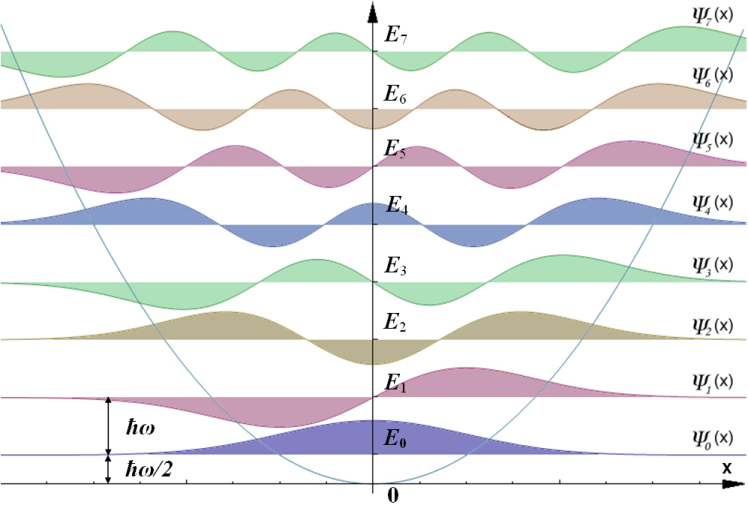
\includegraphics[width=0.7\textwidth]{wavefunctions}
		\caption{First few eigenvectors of the quantum mass-spring system. Image from Wikipedia}
	\end{figure}


\subsection{To Summarize}
The above analysis crucially relied on the Lie brackets $[\hat{H},\hat{C}]$ and  $[\hat{H},\hat{A}]$ and as mentioned before these form what is called the Weyl algebra.
The Weyl algebra is related to another structure in mathematics called the \textbf{Heisenberg Lie algebra}.

 For many other quantum mechanical systems, it turns out that the relevant operators are related to other Lie algebras which satisfy similar Lie bracket identities. And thus the analysis of quantum mechanical systems often reduces finding the correct Lie algebra for the system which allows us to write the quantum mechanical operators in terms of simpler operators. For example, the angular momentum operator is related to Lie algebra $\frak{sl}_2(\C)$ the vector space of $2 \times 2$ matrices with trace 0.

Finally, for a large class of Lie algebras it is known that the eigenvalues of operators are a discrete set and thus the quantization of energy levels is a physical manifestation of the representation theory of Lie algebras.

\end{document}
